\begin{figure*}[!ht]
\centering
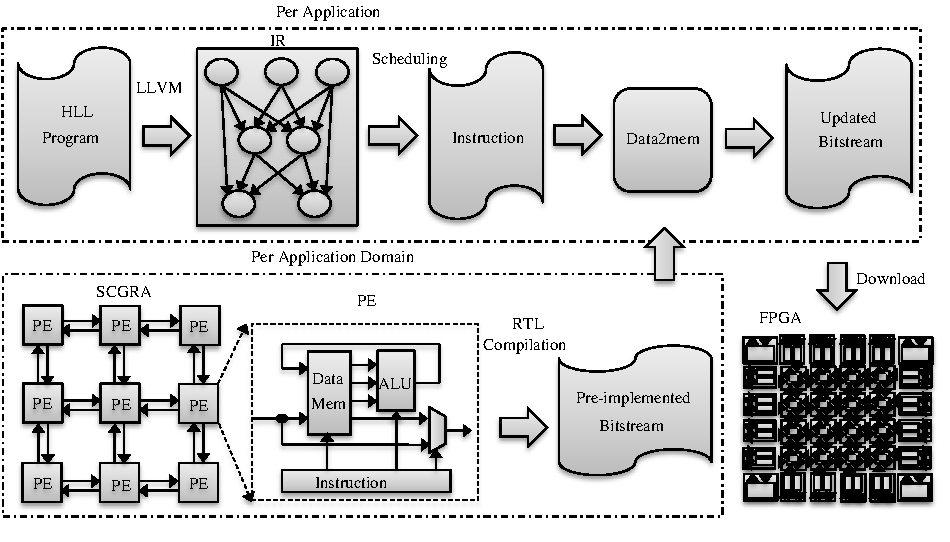
\includegraphics[width=10cm]{designflow}
\vspace{-1em}
\caption{Overview of the proposed soft coarse-grained reconfigurable array based high-level synthesis design methodology.}
\label{fig:design-methodology}
\vspace{-1em}
\end{figure*}

\section{Proposed Design Methodology}\label{sec:methodology}
%\subsection{A Two-Part Design Methodology}
\figref{fig:design-methodology} depicts an overview of the proposed high-level synthesis methodology.  As shown in the diagram, the proposed methodology can be divided into two distinct parts.  The first part, shown in the top half of the figure, is expected to execute frequently.  It should be executed every time a new design iteration is required, a new debug cycle is started, or simply when a new application within the same application domain is implemented.  On the other hand, the second part of the design flow, shown in the bottom half of the figure, is expected to execute infrequently, perhaps on a per-application domain basis.  Towards the end of the top half of the flow, the scheduling result is merged with the pre-built bitstream from the bottom half to produce the final downloadable bitstream for the target FPGA.

\subsection{Per Application Domain Steps}
The goal of the bottom half is to produce a highly optimized SCGRA for the target application domain.  The resulting SCGRA should capture key computational characteristics common to the target application domain.  For example, depending on the application domain, either fixed point number or floating number system may be employed.  The kinds of supported operations in the processing element (PE) may also be fine-tuned at this stage.  For instance, complex mathematical operations may be useful in one application domain while they may be omit to conserve hardware resources in other cases.  Finally, system-wide parameters, such as the number of PE employed, the PE connection topology, I/O bandwidth and data memory size should also be considered.

Note that since the design of the CGRA is soft, it is always possible to implement a different SCGRA as deemed appropriate.  Therefore, the design for the bottom half should be considered a best effort design.  It represents a tradeoff between generality and efficiency -- A generic solution helps to avoid executing the lengthy bottom half, saving compilation time, but will inadvertently consume more hardware resources, impacting the maximum clock frequency of the implementation.  In \secref{sec:scgra}, one class of such SCGRA suitable for our targeted benchmark application will be used to demonstrate how such array can been optimized to execute on extreme frequency of the target FPGA.

\subsection{Per Application Steps}
The goal of the top half of the design flow is to compile the specific user application to execute on the pre-compiled SCGRA.  Since no low-level FPGA implementation tool is involved, the runtime is comparable to common software compilation time of large systems.  This enables significant reduction in application development time so long as the SCGRA has already been implemented.  The reduced compilation time has net effect on increasing number of achievable debug cycles per day, greatly enhancing the productivity of the designers.

There are three sub-steps in the top half.  First, application developed in high-level languages are compiled into an intermediate representation (IR), which in our case, is the data flow graph (DFG) of the compute kernel.  Subsequently, a scheduler is invoked to schedule the DFG onto the SCGRA, taking into account the architectural features.  Finally, based on the scheduling results, the cycle-by-cycle control words for each PE within the SCGRA is generated and merged into the pre-built bitstream from the bottom half, producing the final updated bitstream for download.


%The per application layer targets at the implementation of a specific application. It abstracts IR from HLL program using LLVM \cite{llvm} first. Then it schedules the IR to a pre-implemented SCGRA using a delicate list scheduling algorithm. At the end of the scheduling, the control words that dictate all the activities of the SCGRA are dumped. (Since the control words are used to control the SCGRA cycle by cycle, we also call the control words instructions.) When all the instructions are collected, they are sent to the Xilinx tool data2mem \cite{data2mem} together with the pre-implemented bitstream. Thanks to this ISE independent tool, the instruction memory context of the pre-implmented SCGRA bitstream can be replaced with the new instructions directly and a new bitstream is generated. The new bitstream is actually an implementation of the application and can be downloaded to FPGA. Details of the design methodology will be elaborated in the following sections.


\subsubsection{Applications To IR}
The first step of our compilation process is to process the user application described in high-level languages into a common intermediate representation (IR) for the subsequent scheduling step.  In our current implementation, we have opted to make use of the open source LLVM compiler infrastructure \cite{llvm} for this task.  Apart from having a wide community support, one of the advantages of utilizing LLVM rests on its many readily available front-end for different languages such as C/C++, Java, .NET, Python, etc.  This allows easy extension of our work in the future across many different application domains.  Currently our applications are written in C.

Given an input application, we begin with manually identifying compute kernels that will be accelerated by FPGAs.  Once identified, the compute kernels undergo a series of reshaping to increase the amount of available parallelism.  For this purpose, we have initially opted to fully unroll the inner loops of the compute kernels.  We note that fully unrolling loops may not always be feasible and may not result in an optimal design.  This is left as future extension to this work while we focus on the overall design methodology here.


%The proposed HLS methodology mainly targets at accelerating the computation intensive kernels using FPGA. Typically the computation kernels can be loops with large iterations or functions called repeatedly and it is not applicable to deploy an extensively expanded kernel to FPGA due to the resource constrain and the IO constrain. Meanwhile, the primitive computation kernel body can be light weight and its parallelism is insufficient for FPGA acceleration. In this case, a computation kernel can be appropriately reshaped using techniques such as partial unrolling, such that the entire kernel can be divided into a number of identical kernel bodies and the computation kernel can be accelerated by simply deploying the kernel body to FPGA. When the kernel bodies are independent with each other, arbitrary number of kernel bodies can be put together and the reshaping is pretty simple. When the kernel bodies are dependent with each other, the reshaping problem gets complex. A preliminary solution to this problem is based on modulo scheduling \cite{rau1994iterative}. With modulo scheduling, the operations of the computation kernel can be pipelined. By ignoring the prologue part and epilogue part of the pipeline, the main part of the pipeline can be viewed as a group of identical computation bodies with different scales. Consequently, the computation kernel with dependent kernel bodies can also be reshaped as required. The reshaping scheme is not the focus of the paper and extensive efforts are still needed to figure out an optimal solution, sowe leave this for future study. In this paper, we assume that we are accelerating an computation kernel body. Also note that the term 'computation kernel body' is regarded as 'computation kernel' for the sake of convenience in the following sections. 

%The output DFG describes the data dependency of the HLL program, and helps explore operation parallelism during the SCGRA scheduling step especially for these computation kernels. Hence, it is considered as IR of our HLS methodology. 


The identified compute kernel is subsequently compiled to the machine-independent assembly language of LLVM through its Clang frontend for C/C++ programs.  It is then processed within the LLVM framework in preparation for intermediate DFG generation.  Several LLVM passes, including dead code elimination, loop simplification, and function inline are employed as optimization.  Moreover, branch instructions within the kernel body are merged into simple basic blocks by the introduction of PHI instructions.  Finally, once the code is transformed into static single assignment (SSA) style, it goes through our in-house pass that transforms the LLVM assemble code into a DFG ready for SCGRA scheduling. 

\subsubsection{SCGRA Scheduling}
In the SCGRA scheduling step, a list scheduling algorithm similar to \cite{colinheart} is adopted to schedule the DFG to the SCGRA infrastructure. It statically schedules the entire DFG on the target SCGRA. Such statically scheduled architecture is crucial in keeping the target SCGRA simple and efficient. To adapt to the proposed SCGRA structure, the scheduling metric is delicately adjusted to compromise the communication cost and load balance.

%The basic list scheduling process is relatively straightforward as shown in \algref{alg:sch}. Initially, it constructs an operation list in which all the operations have their source operands ready. Then it goes to the scheduling kernel. In the scheduling kernel, the PE that meets the PE selection metric is selected first. After that, the operation that fits the selected PE best according to the operation selection metric is chosen. As both the PE and the operation are determined, it gets to commit the scheduling, which includes finding the shortest routing paths, moving source operands to target PE along the routing paths and calculating the operation on target PE. Finally, it updates the operation list and repeats the scheduling kernel until the list becomes empty. In this work, we have made a few modifications on PE selection metric and operation selection metric to adapt to the DFG characteristics and the target SCGRA structure.

%\begin{algorithm}
%\caption{The SCGRA scheduling algorithm.}
%\label{alg:sch}
%\begin{algorithmic}
%\PROCEDURE{ListScheduling}
%\STATE Initialize the operation ready list $L$
%\WHILE {$L$ is not empty}
%\STATE select a PE $p$
%\STATE select an operation $l$
%\STATE OPScheduling($p$, $l$)
%\STATE Update $L$
%\ENDWHILE
%\ENDPROCEDURE
%
%\PROCEDURE {OPScheduling($p$,$l$)}
%\FORALL {predecessor operations $s$ of $l$}
%\STATE Find nearest PE $q$ that has a copy of operation $s$
%\STATE Find shortest routing path from PE $q$ to PE $p$
%\STATE Move operation $s$ from PE $q$ to PE $p$ along the routing path
%\ENDFOR
%\STATE Do operation $l$ on PE $p$
%\ENDPROCEDURE
%
%\end{algorithmic}
%\end{algorithm}

%Since each node of the DFG represents an operation and the DFG is actually a fine-granularity task graph, the PEs have much less time slots idle and can be busy all through the scheduling. In this case, we simply set the time interval that PE has been idle as the PE selection metric to find out the PE that guarantees the earliest computation. In addition, we also add PE utilization constrain to narrow down the PE candidates and help the scheduler to keep load balance. At the same time, we notice that the operation number of the DFG typically is much larger than the PE number of the SCGRA. There are sufficient ready operations in the DFG for scheduling and it makes little difference whether the operations on critical paths are executed earlier or later. As the routing cost between PEs is large due to the deep SCGRA pipeline depth and routing distance becomes essential to the scheduling performance, we set the routing cost that it takes the scheduler to move all the source operands to target PE as operation selection metric. Moreover, we also keep all the operand storing records, and each operand may have multiple copies across the CGRA. When an operand is needed for computation, we always fetch the source operand from the nearest PEs to further reduce the routing cost.

%In order to move a source operand to the selected PE, the scheduler must reserve all necessary hardware resources along the entire routing path for each corresponding time slot.  As the SCGRA status is changing through the scheduling process, a determined routing will soon deteriorates the scheduling performance. In this work, we take the time interval that it costs to move an operand from upstream PE data memory to downstream PE data memory as the link weight. Link weight is updated in real time and thus it indicates the routing congestion information of each link. With all the link weight across the SCGRA updated, we further calculate the routing path of a PE pair using Dijkstra algorithm. Since the Dijkstra algorithm here takes both the routing distance and routing congestion information into account, it helps to find out a near optimal routing in real time and is able to provide a fast operation transmission.

%On top of the issues mentioned, the scheduler is also responsible for the data memory management. The data memory management mainly involves two aspects. On the one side, it slightly adjusts the operation selection to reduce the intermediate operands that need to be stored in data memory and to make sure that the data memory does not overflow. In this work, we add an operation selection filter, which removes the operations with larger children operations from operation ready list, to control the data memory requirements. Note that this scheme is not able to precisely adapt the data memory consumption and it also influences the scheduling performance. Fortunately, the experiments show that the primitive data memory capacity is sufficient to fulfill the requirements of the computation kernels even without stringent filtering. 

%On the other side, the data memory manager also needs to generate read/write addresses that will become part of the instructions. Since the data memory requirements are not pressing, a static address generation is adopted. It does not start until the scheduling kernel is completed, so both an operand's read time $\left( tr_1, tr_2,...,tr_m \right)$ and write time $\left( tw_1,tw_2,...,tw_n \right)$ on a data memory can be obtained from scheduling records. Note that $tr_1<tr_2<...<tr_m$ and $tw_1<tw_2<...<tw_n$. In most occasions, $n=1$, but $n \geq 1$ sometimes because the routing path is changing all the time. An address is allocated to the operand at the first time it is stored in the data memory and the address is released at the last time it is referenced through the data memory. Therefore, the lifetime of the operand in the data memory is from $tw_1$ to $tr_m$.

%Upon completion of the scheduling stage, a cycle-accurate schedule of the operation on each PE, as well as the movement of data between the data memory and the PEs in the SCGRA is obtained.  This schedule must then be encoded accordingly and incorporated into the instruction ROM of the SCGRA.

\subsubsection{Bitstream Integration}
The final step in our proposed HSL methodology is to incorporate the instruction for each PE obtained from the scheduling stage with the pre-compiled SCGRA design.  By design, our SCGRA do not have mechanism to load in instruction streams from external memory.  Instead, we take advantage of the reconfigurability of SRAM based FPGAs and stored the cycle-by-cycle configuration words using on-chip ROM.  The content of these instruction ROMs are embedded in the configuration bitstream.  In particular, the organization of the instruction ROM in the place-and-routed SCGRA design is obtained from its XDL file \cite{beckhoff2011xilinx}, which in turn allows us to create the corresponding BMM file.  With this BMM file, the encoded instructions collected from the DFG scheduling may then be incorporated into the pre-implemented bitstream using the data2mem tool from Xilinx \cite{data2mem}.  
While original SCGRA design needs hours to implement, the bitstream updating scheme only costs a few seconds.



